\documentclass[12pt, a4paper]{scrartcl}
\usepackage{float}
\usepackage[utf8]{inputenc}
\usepackage[english, ngerman]{babel}
\usepackage[T1]{fontenc}
\usepackage{graphicx}
\usepackage{subfigure}
\usepackage{amsmath, amssymb}
\usepackage{eurosym}
\usepackage{abstract}
\usepackage{geometry}
\geometry{left=3.5cm, right=2cm, top=2.5cm, bottom=2.5cm}
\usepackage{fancyhdr, lastpage, listings, wasysym, 
	bibgerm, comment, changebar}

\usepackage{xcolor}
%\usepackage[hidelinks]{hyperref}
\usepackage[
		pdfauthor={Christian Högerle, Nico Vinzenz, Felix Waibel},
        pdftitle={Chatbots mit Künstlicher Intelligenz},
        bookmarks=true,
        bookmarksnumbered=true, % Verwendete Bookmarks anzeigen
        colorlinks,   % Farbige Links
        linkcolor=black,
        urlcolor=blue,
        citecolor=black]{hyperref}
    
%ermöglicht die Aneinanderreihung von Fußnoten mit Komma   
\let\oldFootnote\footnote
\newcommand\nextToken\relax

\renewcommand\footnote[1]{%
    \oldFootnote{#1}\futurelet\nextToken\isFootnote}

\newcommand\isFootnote{%
    \ifx\footnote\nextToken\textsuperscript{,}\fi}


%Ermöglicht Zeilenumbrüche in Links (Fußzeile)
\makeatletter
\g@addto@macro\UrlBreaks{\do\-}
\makeatother

\usepackage{color}
\usepackage{colortbl}
\usepackage{acronym}
\usepackage{footnote}
\usepackage{url}

%Global gleiche Anführungszeichen
\usepackage[autostyle=true,german=quotes]{csquotes}

\bibliographystyle{alphadin} 

\title{Künstliche Intelligenz - Warnung vor der Singularität}
\author{Christian Högerle, Nico Vinzenz, Felix Waibel}
\date{\today}

%Absatz mit 6pt und nicht einrücken
\setlength{\parskip}{6pt}
\setlength{\parindent}{0pt} 

\begin{document}
	\pagestyle{empty}
	\begin{figure}[ht]
	\subfigure{
\includegraphics[width=0.45\textwidth]{Bilder/hswgt-logo.jpg}}\hfill
	\subfigure{
\includegraphics[width=0.45\textwidth]{Bilder/master-logo.jpg}}\\[1.5cm]
\end{figure}

\begin{center}
	\textsc{\Large{Hausarbeit Berufsethik\\[1.5cm]}}
\end{center}

\begin{center}
	\LARGE{\textbf{
			Künstliche Intelligenz \\
			Warnung vor der Singularität\\[2.0cm]
	}}
\end{center}

\begin{center}
	\small{im Studiengang Informatik}\\
	\small{in der Fakultät Elektrotechnik und Informatik}\\
	\small{der Hochschule Ravensburg-Weingarten}\\[2.0cm]
\end{center}

\begin{center}
	\large{15. Dezember 2017\\[2.0cm]}
\end{center}

\begin{center}
	\begin{tabular}{lll}
		\textbf{Vorgelegt von:}\\
		 & & Felix Waibel\\
		&& Christian Högerle\\
		&& Nico Vinzenz
	\end{tabular}
\end{center}
	\section*{Eidesstattliche Erklärung}
Diese Hausarbeit wurde von uns selbstständig verfasst. Es wurden nur die angegebenen Quellen und Hilfsmittel verwendet. Alle wörtlichen und sinngemäßen Zitate sind in dieser Arbeit als solche kenntlich gemacht.\\

\vspace{3cm}
\begin{tabular*}{\textwidth}{c@{\extracolsep\fill}cc}
	\cline{1-1}
	\cline{3-3}
	\\
	\ \ \ \ \ \ \ \ \ Ort, Datum\ \ \ \ \ \ \ \ \ \ & & \ \ \ \ \ \ \ \ \ Unterschrift\ \ \ \ \ \ \ \ \ \\
\end{tabular*}

\vspace{3cm}
\begin{tabular*}{\textwidth}{c@{\extracolsep\fill}cc}
	\cline{1-1}
	\cline{3-3}
	\\
	\ \ \ \ \ \ \ \ \ Ort, Datum\ \ \ \ \ \ \ \ \ \ & & \ \ \ \ \ \ \ \ \ Unterschrift\ \ \ \ \ \ \ \ \ \\
\end{tabular*}

\vspace{3cm}
\begin{tabular*}{\textwidth}{c@{\extracolsep\fill}cc}
	\cline{1-1}
	\cline{3-3}
	\\
	\ \ \ \ \ \ \ \ \ Ort, Datum\ \ \ \ \ \ \ \ \ \ & & \ \ \ \ \ \ \ \ \ Unterschrift\ \ \ \ \ \ \ \ \ \\
\end{tabular*}
	\vspace*{\fill}
\begin{abstract}
	\noindent

\end{abstract}

	\section*{Abkürzungsverzeichnis}
\begin{acronym}
	\acro{KI}{Künstliche Intelligenz}
\end{acronym}
	\tableofcontents
	\clearpage
	%Seitenzahl und Kapitelname in der Kopfzeile anzeigen
	\pagestyle{fancy}
	\fancyhf{}
	\pagenumbering{arabic}
	\fancyhead[RO,LE]{\small \sffamily  \thepage}
	\fancyhead[LO,RE]{\small \sffamily \leftmark}
	\section{Einleitung}


\subsection{Motivation}

\subsection{Fragestellung}


\subsection{Problemstellung}
	\section{Grundlagen}
In diesem Kapitel werden kurz \ac{ki} sowie Chatbots beschrieben.
Daraufhin werden die drei Philosophen Platon, Aristoteles und Nietzsche vorgestellt, deren Ethiken in Kapitel 3 genauer betrachtet und bewertet werden.

\subsection{Künstliche Intelligenz}
Bereits viele Menschen haben sich daran versucht den Begriff der \ac{ki} zu definieren. Leider gibt es bislang keine allgemein anerkannte und eindeutige Definition. Bereits bei der Frage \enquote{Was ist Intelligenz} gibt es nicht eine einzig wahre Aussage\footnote{vgl. \cite{Intelligenz}}. Sicher ist, die Menschen nehmen eine besondere Stellung unter den Lebewesen ein. Diese besondere Stellung basiert unter anderem auf unserer Intelligenz. 

Der \ac{ki} Pionier John McCarthy veröffentlichte bereits 1955 ein Exposé in dem er auf die Künstliche Intelligenz eingeht. Das Exposé definiert die \ac{ki} wie folgt:
\begin{quote}
		\glqq For the present purpose the artificial intelligence problem is taken to be that of making a machine behave in ways that would be called intelligent if a human were so behaving\grqq.\footnote{\cite{PROPOSALMcCarthy}}
\end{quote}
Diese Definition ist allerdings zu vage. Denn für viele Menschen gilt ein Roboter, der einem Hindernis ausweicht schon als intelligent. Für Informatiker ist das Ausweichen eine logische Schlussfolgerung aus eingehenden Sensorsignalen. Bekommt der Roboter die Sensoreingabe, dass er vor einem Hindernis steht, so ändert dieser aufgrund der Programmierung die Richtung.

Einen weiteren Versuch die \ac{ki} zu definieren unternahm Elanie Rich bereits 1983:
\begin{quote}
	 \glqq Artificial Intelligence is the study of how to make computers do things at which, at the moment, people are better\grqq.\footnote{\cite{ArtificialIntelligence}}
\end{quote}

Das nächste Beispiel nennt eine \glqq Sache\grqq , in der Computer uns überlegen sind. 
Grundsätzlich sind diese im Speichern von Daten und der Berechnung von nummerischen Aufgaben leistungsfähiger als wir. 
Beim Erkennen von Objekten sind jedoch wir Menschen aktuellen Algorithmen noch weit überlegen. 

Sobald wir einen Raum betreten findet in unserem Unterbewusstsein eine Objekterkennung statt. Wir erkennen sofort, dass der Raum beispielsweise drei Fenster, zwei Türen und vier Wände hat. Gleichzeit erkennen wir Gegenstände im Raum wie Tische, Stühle und Monitore. Dadurch schließen wir darauf, dass dieser Raum ein Computerraum sein muss. Dieser Entschluss wird gefasst mit Hilfe von Wissen, welches wir bereits besitzen und Erfahrungen, die wir bereits gemacht haben. Wir verknüpfen im Bruchteil einer Sekunde die Objekte mit unserem bereits vorhandenem Wissen um einen Entschluss zu fassen.

Die aktuelle \ac{ki} steckt hier noch in den Anfängen. 
Moderne Algorithmen können zwar mehr oder weniger gut Objekte erkennen und diese Greifen, ihre zugrundeliegende \ac{ki} kann sich jedoch kein Gesamtbild der Umgebung machen.
Die beiden vorherigen Beispiele sollen verdeutlichen, dass es sowohl Dinge gibt, die ein Computer aktuell besser kann, aber auch Dinge gibt, die ein Computer noch nicht annäherungsweise so gut kann wie ein Mensch.

Die \ac{ki}-Forschung ist ständig im Wandel. Gilt ein Problem für sie als gelöst, so verschieben sich ihre Aufgabenbereiche.  
Wie sich diese verändern zeigen zwei Beispiele. Im Jahr 1997 schlägt IBM's Deep Blue den Schach Weltmeister Garri Kasparow\footnote{vgl. \cite{SchachQuelle}}. Dies hatte zur Folge, dass die \ac{ki}-Forschung nach und nach das Interesse an Schach verlor. Aus ihrer Sicht gilt Schach im Bezug zu \ac{ki} heute als gelöst.

Anfang 2016 gab es eine weitere Sensation. Die \ac{ki} Alpha Go von Google schlägt einen menschlichen Go-Profi\footnote{vgl. \cite{GoQuelle}}. Auch diese Entwicklung ist ein Grund dafür, dass sich die \ac{ki}-Forschung auf neue Aufgabenbereiche konzentrieren wird. 

Es gibt noch zahlreiche Gebiete, in denen wir Menschen der \ac{ki} weit überlegen sind. Durch die rasante Entwicklung der letzten Jahre in der \ac{ki} werden immer mehr Anwendungen und Produkte mit ihr verknüpft. So setzen Unternehmen bereits sogenannte Chatbots (\ac{ki}-basierte Dialogsysteme) zur Kundenkommunikation ein.

\subsection{Chatbot}
Ein Chatbot ist eine Art Maschine für die Kommunikation mit dem Menschen. Meistens besitzt ein Chatbot ein Dialogsystem, sprich der Kommunikationspartner kann per Texteingaben mit dem Chatbot kommunizieren. 
Der Mensch stellt zunächst eine Frage per Texteingabe. Daraufhin versucht der Chatbot diese Frage zu interpretieren und generiert eine Antwort.

Die Idee eine Maschine zur Kommunikation mit dem Menschen einzusetzen ist nicht neu. Bereits 1966 entwickelte Joseph Weizenbaum ein Computerprogramm, das die Kommunikation mit Mensch und Computer ermöglichte. Das Programm wird \glqq ELIZA\grqq\ genannt. Im Hintergrund verwendet das Programm ein sogenanntes \glqq Pattern Matching\grqq\, was einer Mustererkennung entspricht. Mit dieser eigentlich einfachen Technik war es möglich den ersten Chatbot zu programmieren. 

Eine einfache Version von ELIZA verwendet einen Thesaurus. Dies ist eine Art Wörterbuch, dessen Wörter durch Relationen miteinander verbunden sind. So ist zum Beispiel Mutter mit dem Wort Familie verbunden. Des Weiteren gibt es ein vordefiniertes Set von Phrasen. Diese Phrasen sind häufig Fragen oder Aufforderungen. Ein Beispiel ist auf der deutschen Wikipedia-Seite zu finden\footnote{vgl. \cite{WikiELIZADE}}. 
\begin{quote}
    Benutzer: Ich habe ein Problem mit meinem Vater.\newline
    ELIZA: Erzählen Sie mir mehr über Ihre Familie! 
\end{quote}
Hier sieht man wie das Wort \glqq Vater\grqq\ mit dem Wort \glqq Familie\grqq\ in einer Relation steht. ELIZA verwendet dann eine passende Phrase zum Wort \glqq Familie\grqq.
\begin{quote}    
    Benutzer: Krieg ist der Vater aller Dinge.\newline
    ELIZA: Erzählen Sie mir mehr über Ihre Familie!
\end{quote}    
Im zweiten Beispiel verwendet ELIZA die gleiche Phrase wie im ersten Beispiel. An dieser Stelle kann man sehr gut sehen, dass ELIZA die Bedeutung des Satzes in keinster Weise versteht. Es wird rein nach \glqq Pattern Matching\grqq\ vorgegangen. Es wird eine passende Phrase zu einem passendem Pattern gesucht.\footnote{vgl. \cite{WikiELIZADE} und \cite{WikiELIZA}}    

Heute setzen immer mehr Firmen Chatbots in der Kundenkommunikation ein, speziell beim Support von Kunden. So greifen Firmen wie Lufthansa, Zalando, Opel, etc. bereits auf Chatbots zurück. 
Diese sind zwar noch nicht voll integriert, erste Experimente um dies zu erreichen finden aber bereits statt.\footnote{vgl. \cite{UnternehmenChatbots}}

Lufthansa startete beispielsweise im November 2016 den Chatbot \glqq Mildred\grqq. Dieser Chatbot ermöglicht die Suche nach dem günstigsten Preis für einen Flug. Die angebotenen Flüge liegen alle innerhalb der kommenden neun Monate. Der Chatbot ist in den Facebook-Messenger integriert. Für eine Suche geben die Nutzer Abflug- und Zielflughafen an. Auch die internationalen Buchstabencodes können verwendet werden. Der Chatbot erkennt auch die Buchungsklassen der Lufthansa. Über die mobile Version von LH.com kann dann das angebotene Ticket gebucht werden. 

Erste Tests des Chatbots offenbarten jedoch bereits Schwächen. Auf die Frage \glqq Kann ich am selben Tag zurück?\grqq\ entgegnet Mildred, ob sie nochmals Flüge suchen soll. Eine weitere Eingabe lautet \glqq Ich habe Flugangst\grqq, Mildred fragt daraufhin \glqq Wohin möchtest du fliegen?\grqq. Wie diese Beispiele zeigen ist Mildred noch weit entfernt davon, eine richtige Konversation zu führen. Mit allem was über eine einfache Fluganfrage hinausgeht ist Mildred schlicht überfordert.\footnote{vgl. \cite{LHQuelle1} und \cite{LHQuelle2}} 

Getrieben durch die Fortschritte in der \ac{ki} werden die Chatbots allerdings immer besser. Vor allem der Einsatz maschinellen Lernens hilft dabei kontinuierlich Fortschritte zu erzielen. Es wird immer schwieriger den Gegenüber als Chatbot zu identifizieren. Die University of Reading führte 2014 den sogenannten Turing-Test\footnote{Der Bericht definiert den Test als bestanden: Wenn ein Chatbot für mehr als 5 Minuten für einen Menschen gehalten wird und wenn mehr 30 \% der Testteilnehmer getäuscht werden} beim Chatbot \glqq Eugene Goostman\grqq\ durch. Der Chatbot schaffte es 33 \% der 30 Testteilnehmer zu täuschen.\footnote{vgl. \cite{UnivOfReading}}

Bitkom untersuchte mit Hilfe einer Umfrage den Einsatz von Chatbots unter den Bundesbürgern. Die Umfrage wurde am 18.01.2017 mit dem Titel \glqq Jeder Vierte will Chatbots nutzen\grqq\ veröffentlicht\footnote{vgl. \cite{BitkomChatbot}}. Es wurden im November 2016 insgesamt 1.005 Personen ab 14 Jahren in Deutschland befragt. 

Die Umfrage kam zu interessanten Ergebnissen:
\begin{itemize}
	\item Sieben von zehn Befragten können sich vorstellen einen Chatbot zu verwenden. Zum Beispiel für die Terminplanung, 	beim Ticketeinkauf oder beim Online-Shopping.
\end{itemize}
Unter denen, die keine Chatbots verwenden wollen:
\begin{itemize}	
	\item Gaben 63 Prozent an, dass sie nicht mit einer Maschine kommunizieren wollen. 
	\item Etwa 50 Prozent bezweifeln, dass Anfragen zuverlässig bearbeitet werden können.
	\item 47 Prozent denken, dass Chatbots uninteressant sind, weil die \ac{ki} noch nicht ausgereift ist.
\end{itemize}
Dieser Auszug aus der Studie zeigt uns, dass die Befragten mit etwa 70 Prozent hinter dem Einsatz von einem Chatbot stehen. Sie könnten es sich vorstellen, einen Chatbot auch für private Angelegenheiten zu verwenden. Wie sich dieses Gefüge mit der Zeit verändern wird kann jedoch noch keiner sagen.  

\subsection{Platon}
Platon (* 427 v.  Chr. in Athen - † 347 v. Chr. in Athen) war ein griechischer Philosoph, der auf die gesamte Entwicklung der Philosophie einen großen Einfluss hatte. 

Platon war Schüler des Sokrates und Überbrachte dessen Gedankengut an die Nachwelt. Selbst gründete er die sogenannte Akademie, in der er Philosophen unterrichtete. Einer seiner bekanntesten Schüler war Aristoteles, der ihm jedoch in zentralen Fragen widersprach. In den Gebieten der objektiv-idealistischen Philosophie, der Metaphysik, der Erkenntnistheorie, der Ethik, der Anthropologie, der Staatstheorie, der Kosmologie, der Kunsttheorie und der Sprachphilosophie war er richtungsweisend für sehr viele Philosophen. Der Mittelpunkt seiner Philosophie bildet die Ideenlehre.\footnote{vgl. \cite{Platon1} \cite{Platon2}}

\begin{figure}[H]
	\centering 
	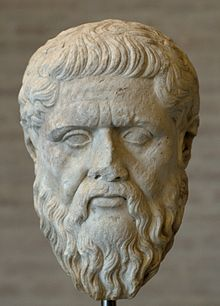
\includegraphics[width=0.4\textwidth]{Bilder/kap3/platon} 
	\caption{Römische Kopie eines griechischen Platonporträts.\cite{WikiPL}  \label{portraitPlaton}}
\end{figure}

\subsection{Aristoteles}
Aristoteles (* 384 v. Chr. in Stagira (Griechenland) - † 322 v. Chr. in Chalkis) war Wissenschaftler, Biologe, Physiker und Philosoph. 

Als Sohn eines reichen Arztes war es ihm möglich Platons Akademie zu besuchen. Er befasste sich zunächst mit mathematischen und dialektischen Themen. Nach und nach begann er mit der Verfassung von eigenen Werken. Aristoteles blieb etwa 20 Jahre an der Akademie als Student und später als Lehrer. Nach dem Tod Platons verließ er Athen und seine sogenannten \glqq Reisejahre\grqq\ begannen. 
Während der Reisejahre ging Aristoteles auf Einladung von König Philipp II. nach Mieza. 
Dort unterrichtete er seinen Sohn Alexander, der im Laufe der Geschichte unter dem Namen \enquote{Alexander der Große} bekannt werden wird. Sein Weg führte ihn nun wieder nach Athen. Er forschte und lehrte an einem öffentlichen Gymnasium. Nachdem er sich von Alexander dem Großen und dem Königshaus abwandte, wurde ihm Gotteslästerung vorgeworfen. Daraufhin verließ er Athen und zog nach Chalkis. Dort starb er im Oktober 322 v. Chr.. 

Aristoteles zählt bis heute noch zu den bekanntesten und einflussreichsten Philosophen und Naturforschern. Zu den berühmtesten Werken des Aristoteles zählen seine Poetik, Politik und Metaphysik.\footnote{vgl. \cite{Aristoteles1} und \cite{Aristoteles2}}
\begin{figure}[H]
\centering 
 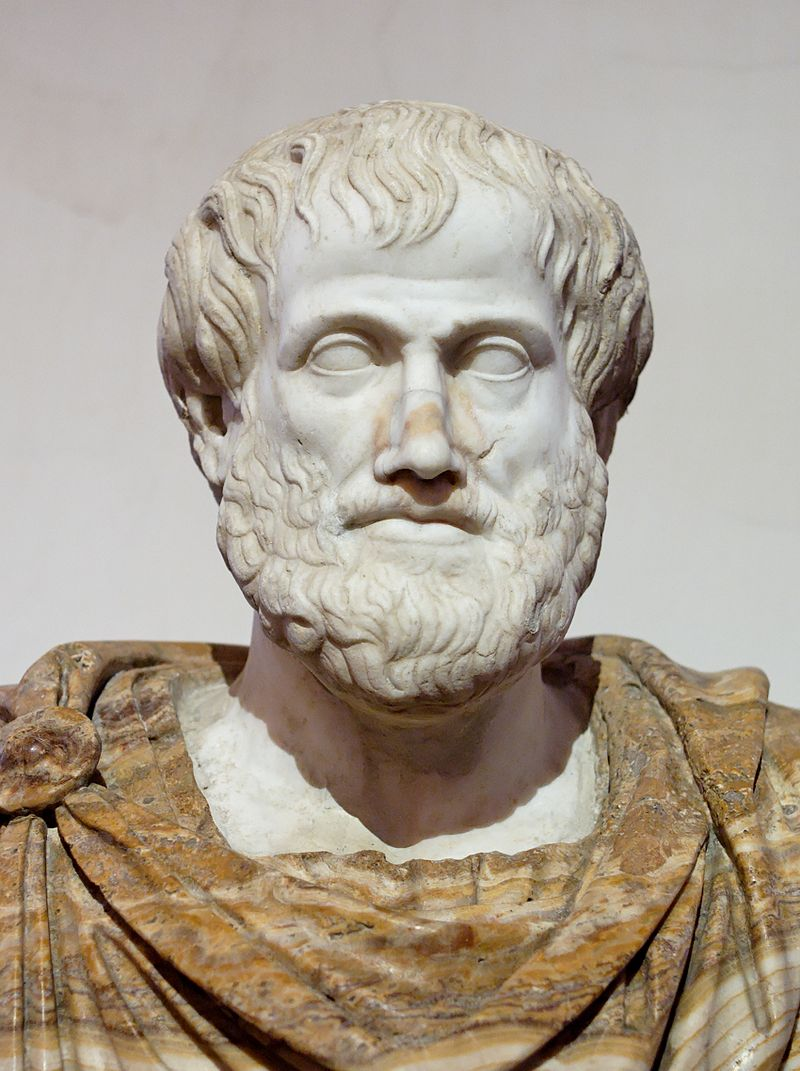
\includegraphics[width=0.4\textwidth]{Bilder/kap3/Aristoteles} 
 \caption{Römische Kopie nach einer Skulptur des Bildhauers Lysippos.\cite{WikiAR}  \label{portraitAristotles}}
\end{figure}

\subsection{Friedrich Nietzsche}
Friedrich Wilhelm Nietzsche (* 15. Oktober 1844 in Röcken - † 25. August 1900 in Weimar) war ein deutscher klassischer Philologe.

Bereits in seiner Jugendzeit fiel er durch überdurchschnittliche sprachliche sowie musikalische Fähigkeiten auf.
Während seines Studiums der klassischen Philologie sowie Theologie in Bonn und Leipzig beschäftigte er sich ausgiebig mit den Werken\footnote{Maßgeblichen Einfluss auf ihn hatte Schopenhauers Hauptwerk \enquote{Die Welt als Wille und Vorstellung}. vgl. \cite{Schopenhauer1}}
des Philosophen Arthur Schopenhauers, die durch ihren Pessimismus seine Weltanschauung nachhaltig beeinflussten.
Des Weiteren übte auch Richard Wagner, Komponist und Freund Nietzsches, Einfluss auf sein Denken aus.

Nach dem Studium der klassischen Philologie sowie Theologie wurde er bereits im Alter von 25 Jahren zum Professor an die Universität Basel berufen.
Aufgrund körperlicher Beschwerden legte er nach 10 Jahren seine Professur nieder und widmete sich daraufhin weitestgehend von Mitmenschen isoliert vollkommen der Philosophie.
Weitere 10 Jahre vergingen bis sich sein körperlicher und psychischer Zustand soweit verschlechterte, dass er zu einem Pflegefall wurde und schlussendlich starb.

Durch seine philosophischen Schriften, darunter sein Hauptwerk \enquote{Also sprach Zarathustra}, erlangte Nietzsche postum Weltberühmtheit.\footnote{vgl. \cite{Nietzsche1}, \cite{Nietzsche2}, \cite{Nietzsche3} und \cite{Nietzsche4}}

\begin{figure}[H]
\centering 
 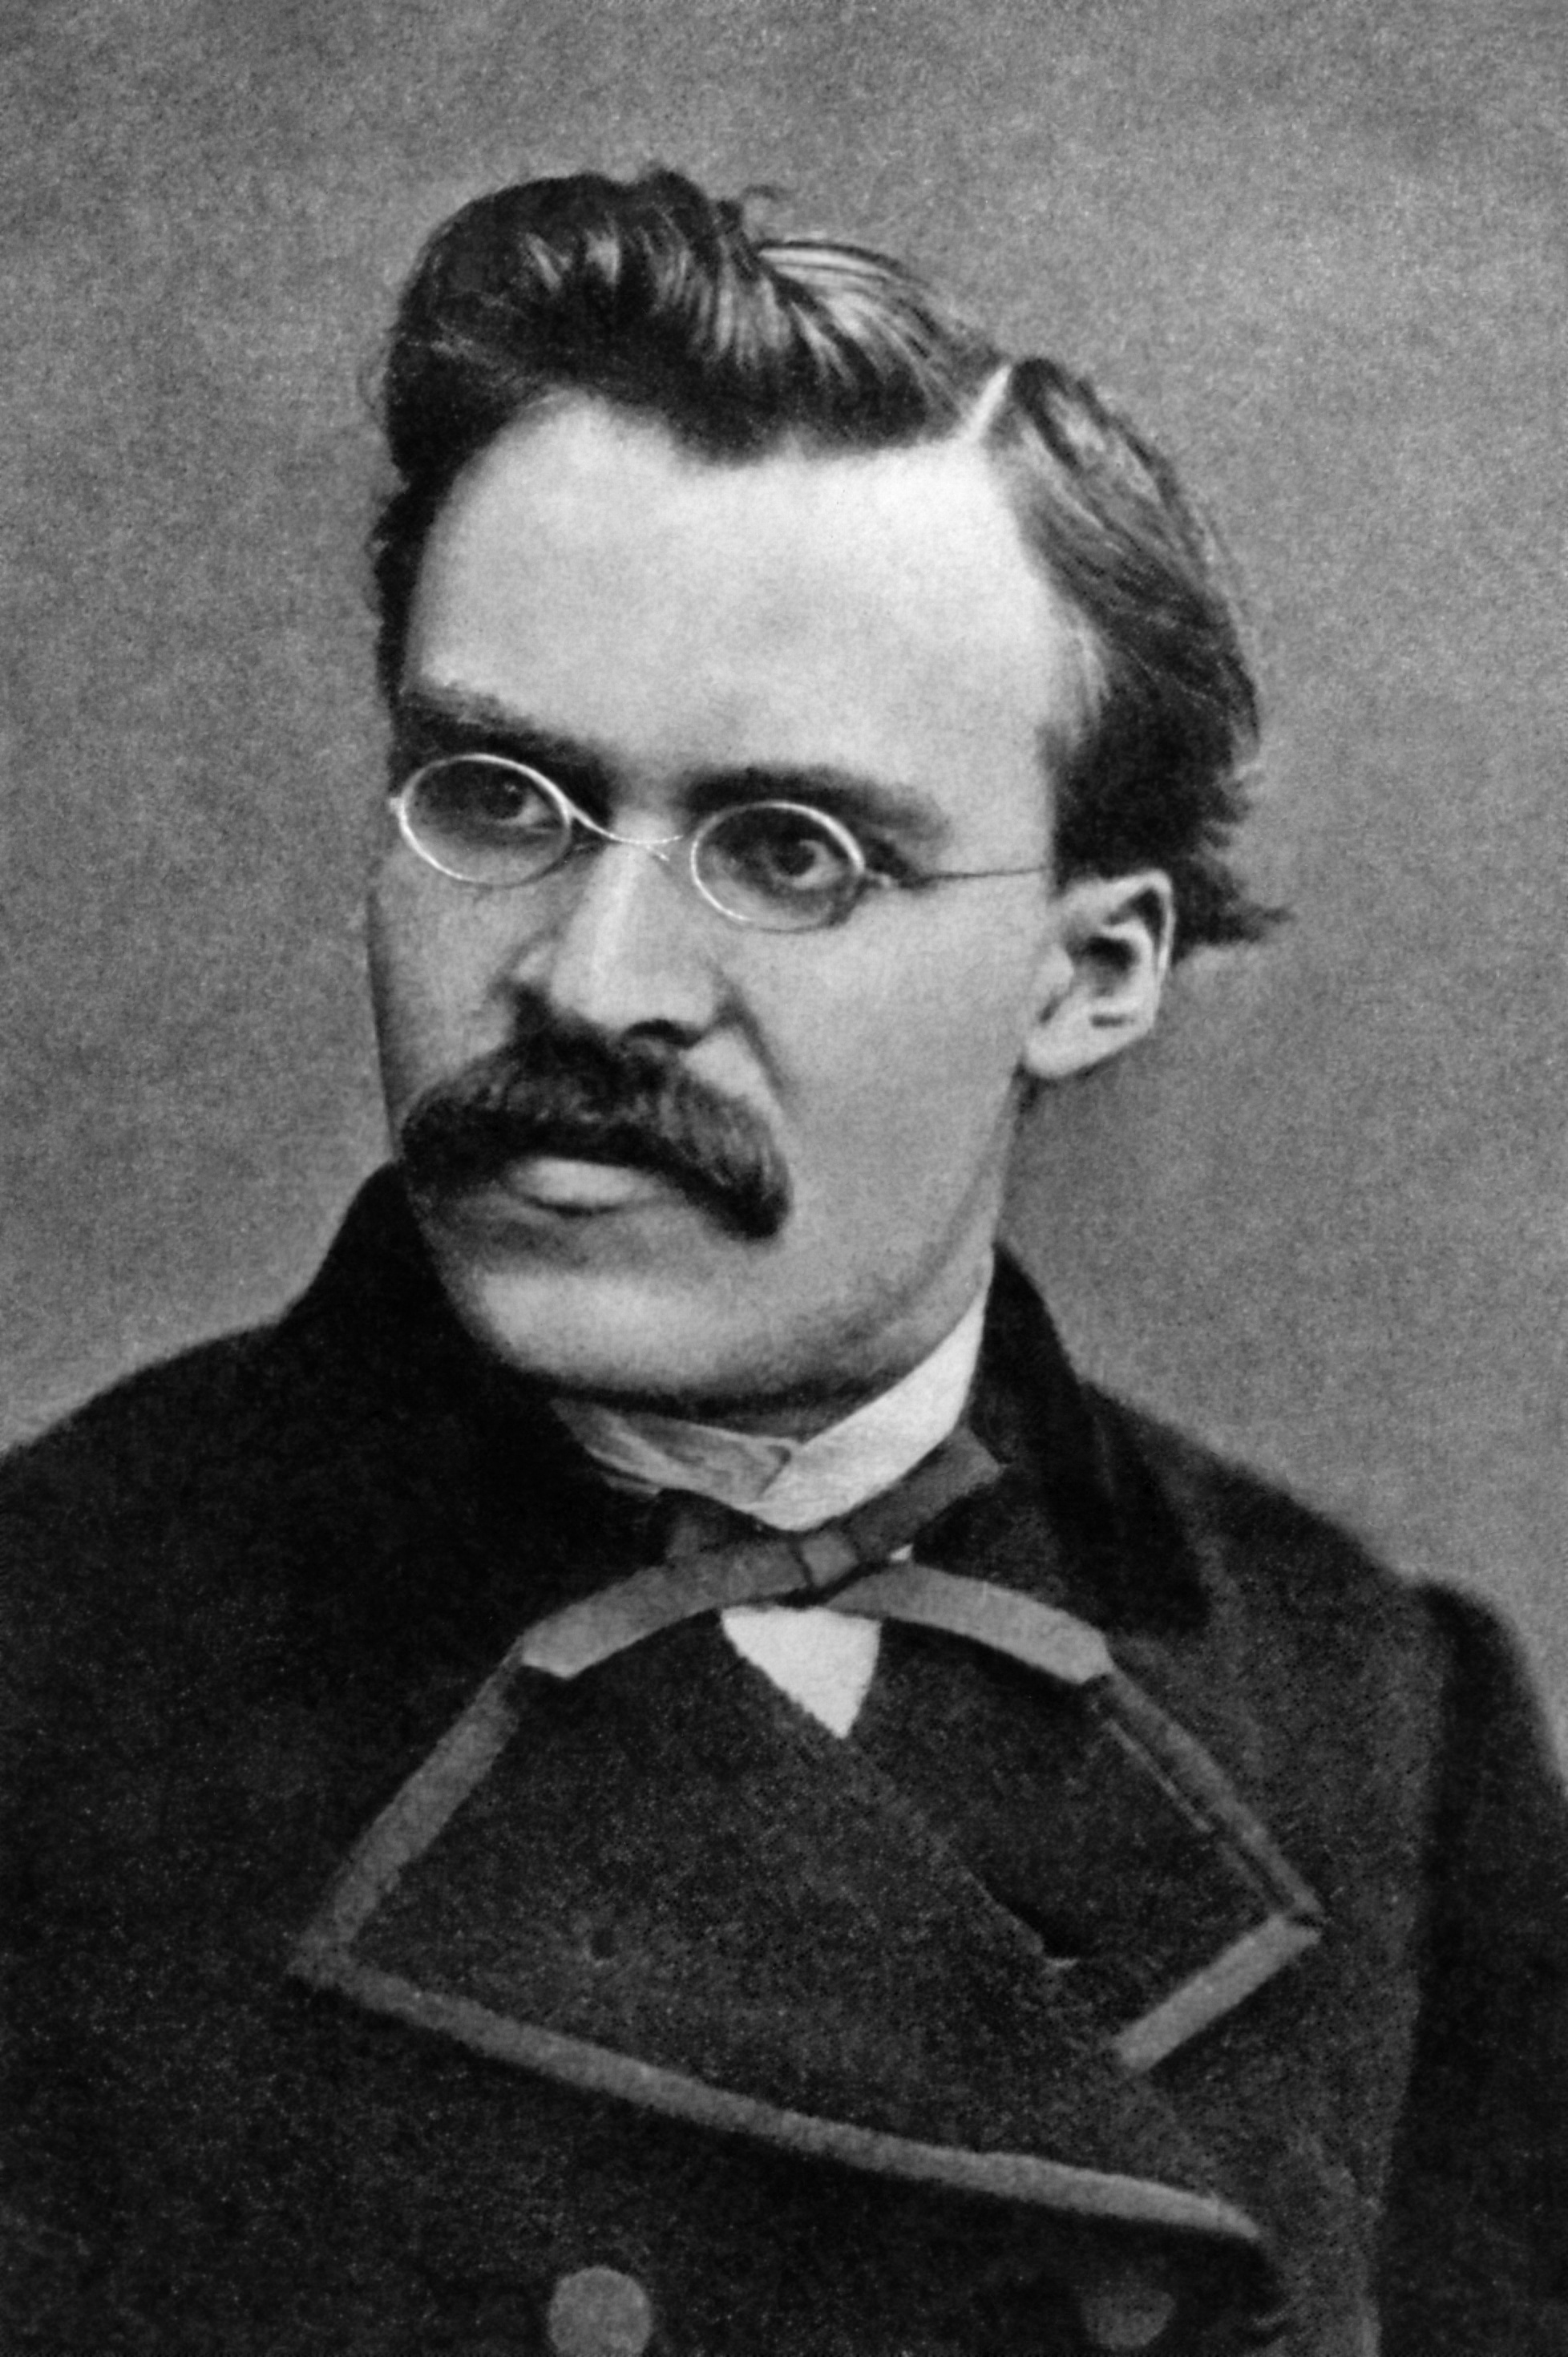
\includegraphics[width=0.4\textwidth]{Bilder/kap3/nietzschePortrait} 
 \caption{Friedrich Nietzsche um 1869.\cite{WQ14}  \label{portraitNietzsche}}
\end{figure}





	\section{Ethiken}
In diesem Kapitel möchten wir drei verschiedene Ethiker und ihre Kernthesen vorstellen. Außerdem gehen wir darauf ein wie diese den Einsatz von Chatbots bewerten könnten. Dazu sei gesagt, dass es dazu nicht die richtige Antwort gibt. Wir versuchen unsere Aussagen anhand von Gedanken der Ethiker zu belegen. 


\subsection{Platon}
Platon war ein griechischer Philosoph, der auf die gesamte Entwicklung der Philosophie einen großen Einfluss hatte. Geboren wurde Platon 427/428 \ac{vCHR} in Athen, wo er auch 80 Jahre später, im Jahre 347 \ac{vCHR}, verstarb. Er war Schüler des Sokrates und Überbrachte dessen Gedankengut an die Nachwelt. Selbst gründete er die sogenannte Akademie, in der er selbst Philosophen unterrichtete. Einer seiner bekanntesten Schüler war Aristoteles, der ihm jedoch in zentralen Fragen widersprach.  In den Gebieten der objektiv-idealistischen Philosophie, der Metaphysik, der Erkenntnistheorie, der Ethik, der Anthropologie, der Staatstheorie, der Kosmologie, der Kunsttheorie und der Sprachphilosophie war er richtungsweisend für sehr viele Philosophen. Der Mittelpunkt seiner Philosophie bildet die Ideenlehre.\footnote{vgl. \url{http://www.whoswho.de/bio/platon.html} abgerufen am 28.11.2018}

\begin{figure}[H]
	\centering 
	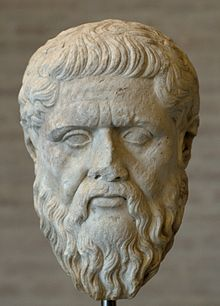
\includegraphics[width=0.3\textwidth]{Bilder/kap3/platon} 
	\caption{Platonportrait  \label{portraitPlaton}}
\end{figure}

\subsubsection{Kernthesen}

\textbf{Wahrnehmung ist ungleich Wissen}\\[0.3cm]
Nach Platon ist die Wahrnehmung unserer fünf Sinne (sehen, hören, riechen, schmecken, fühlen) ungleich Wissen. Dies beweist er dadurch, dass Sinne Mängel aufweisen können. Ein Beispiel hierfür wären optische Täuschungen. Das Wissen wird laut ihm jedoch durch unsere Seele mit eigener Kraft  und denken erlangt. Wohingegen die Wahrnehmungen zwar von der Seele aufgenommen und verknüpft werden aber man durch sie keine Erkenntnis oder sicheres Wissen  erlangen kann.

\textbf{Der Ursprung der Ideen}\\[0.3cm]
Hier unterscheidet Platon zwischen zwei Arten der Gleichheit.\\
Zum Einen die Gleichheit der Dinge, hier entscheiden wir mit unseren Sinnen ob zwei Gegenstände gleich sind oder nicht. Wir können so einen Apfel von einer Birne unterscheiden oder feststellen, dass ein Smartphone gleich einem weiteren Smarphone ist.\\
Zum Anderen die Gleichheit an sich, diese findet in unserem Gehirn statt. Hier werden die Vorstellungen von Dingen miteinander verglichen.\\
Das Beispiel mit den gleichen Smartphones zeigt dies sehr deutlich, dreht man eines um, ist die Gleichheit der Wahrnehmung anders. Die Gleichheit in unserer Vorstellung jedoch nicht. Daraus schließt Platon, dass die Vorstellung der Gleichheit gegenüber der Wahrnehmung der Gleichheit besser ist. Wenn man das feststellen kann, so Platon, muss man die Gleichheit an sich schon vorher gekannt haben. Und daraus schließt er, dass wir unsere Ideen schon vor der Geburt in uns haben, sie dann aber verlieren und sie im Laufe des Lebens zurück gewinnen und uns wieder daran erinnern müssen.\\

\textbf{Ideenerkenntnis und Wissenschaft}\\[0.3cm]
Platon veranschaulicht die Ideenerkenntnis und Wissenschaft an Gleichnissen. Diese werden in drei Stufen eingeteilt. Die Welt der sinnlichen Wahrnehmung (das Sichtbare), die Welt des Denkbaren (die Wissenschaft) und die Welt des Erkennbaren (die Vernunft). Nur in der letzten Stufe kann ein Mensch zur Erkenntnis kommen. Die letzte Welt beinhaltet das Reich der Ideen, dort liegt all das Wissen das wir vor der Geburt haben.\\
	
\subsubsection{Meinungsfindung}
Abschließend möchten wir diese Thesen verwenden, um eine mögliche Sichtweise Platons zu diesem Thema zu erörtern.\\[0.3cm]
Zunächst erläutern wir hierzu die Aufgabe eines Chatbots mit künstlicher Intelligenz. Ein Chatbot wird häufig als Fragebeantworter im Kundenservice eingesetzt. Somit gibt er aus seiner künstlichen Welt Informationen weiter, die ein Mensch auf der anderen Seite des Monitors entgegennimmt.\\[0.3cm]
Nehmen wir hierfür die These von Platon, dass Wahrnehmung ungleich Wissen ist. Da die Informationen nicht selbstständig durch eigene Kraft oder  nachdenken gewonnen wurden, sonder durch den Sehsinn, kann die Information kein Wissen sein. Ist aber nicht gerade das der Grund, warum mit dem Chatbot kommuniziert wird? Der unwissende Mensch möchte sich in diesem Szenario Wissen, das er nicht hat, aneignen. Anstatt selbst nachzudenken, geht er den bequemeren Weg, indem er den Chatbot fragt und wird womöglich, wie Platon beschrieb, von seinen Sinnen getäuscht.\\[0.3cm]
Beziehen wir die These des Ursprungs der Ideen mit ein, wird die Sachlage schon schwieriger. Laut Platon haben wir die Ideen vor unserer Geburt in uns, verlieren sie bei der Geburt und müssen uns im  Laufe des Lebens wieder an sie erinnern. Das eine externe Hilfe hierbei behilflich sein darf oder überhaupt kann, sieht diese These nicht vor.\\
Um nun die Ideenerkenntnis und Wissenschaft einzubeziehen, müssen wir uns hier im klaren sein, auf welcher Stufe wir uns hier befinden. Ganz kritisch betrachtet liegt der Chatbot mit künstlicher Intelligenz in der Welt der sinnlichen Wahrnehmung, wie bereits in der ersten These feststellt werden kann. Geht man einen Schritt weiter kann behauptet werden, das der Chatbot in der Stufe der Wissenschaft anzusiedeln ist, da er aus mathematischen Funktionen besteht. Aber auch in dieser Stufe kann er den Menschen nicht zu Erkenntnis führen, dies geschieht erst in der Welt des Erkennbaren. Hierfür müsste man die Behauptung aufstellen, der Chatbot wäre in der Vernunft einzuordnen und wäre eventuell eine Informationsleitung aus dem Reich der Ideen um die Menschen daran zu erinnern, was sie vor der Geburt wussten.\\[0.3cm]
\textbf{Die Konklusion} ist nun, dass Platon wohl keinen Chatbot mit künstlicher Intelligenz als Wissensquelle nutzen würde. Vermutlich würde er die Informationen, die der Chatbot  weiter gibt gar nicht als Wissen ansehen. Wahrscheinlich würde er auch diesen Informationen, die von der Wahrnehmung aufgenommen werden, nicht vertrauen, denn diese täuschen oftmals. Er könnte auch den Weg, sich Wissen von etwas anderem anzueignen als seinen eigenen Gedanken, nicht unterstützen. Den sonst wäre es in seinen Augen kein Wissen und man würde als Mensch nie zur Erkenntnis gelangen. Was wiederum seinen Sinn des Lebens darstellt.     







	%\section{Ethik 2}
\subsection{Friedrich Nietzsche}
%TODO Kompletter Text sprachlich nachbearbeiten und mit Quellenangaben ergänzen.
Friedrich Wilhelm Nietzsche (* 15. Oktober 1844 in Röcken – † 25. August 1900 in Weimar) war ein deutscher klassischer Philologe.

Bereits in seiner Jugendzeit fiel er durch überdurchschnittliche sprachliche sowie musikalische Fähigkeiten auf.
Während seines Studiums der klassischen Philologie sowie Theologie in Bonn und Leipzig beschäftigte er sich ausgiebig mit dem Werk
\footnote{Maßgeblichen Einfluss auf ihn hatte Schopenhauers Hauptwerk \enquote{Die Welt als Wille und Vorstellung}. vgl. \url{http://www.philosophenlexikon.de/arthur-schopenhauer/}, abgerufen am 28.11.2017}
des Philosophen Arthur Schopenhauers, die seine Weltanschauung nachhaltig beeinflussten.
Des Weiteren übte auch Richard Wagner, Komponist und Freund Nietzsches, Einfluss auf sein Denken aus.

Nach dem Studium der klassischen Philologie sowie Theologie wurde er bereits im Alter von 25 Jahren zum Professor an die Universität Basel berufen.
Aufgrund körperlicher Beschwerden legte er nach 10 Jahren seine Professur nieder und widmete sich daraufhin weitestgehend von Mitmenschen isoliert der Philosophie.
Weitere 10 Jahre vergingen bis sich sein körperlicher und psychischer Zustand soweit verschlechterte, dass er ein Pflegefall wurde und schlussendlich starb.

Durch seine philosophischen Schriften, darunter sein Hauptwerk \enquote{Also sprach Zarathustra}, erlangte Nietzsche postum Weltberühmtheit.\footnote{vgl. \url{http://www.philosophenlexikon.de/friedrich-nietzsche-1844-1900/}, abgerufen am 28.11.2017}\footnote{vgl. \url{https://www.was-war-wann.de/personen/friedrich-nietzsche.html}, abgerufen am 28.11.2017}\footnote{vgl. \url{http://www.whoswho.de/bio/friedrich-nietzsche.html}, abgerufen am 28.11.2017}\footnote{vgl. \url{https://www.dhm.de/lemo/biografie/friedrich-nietzsche}, abgerufen am 28.11.2017}

\begin{figure}[H]
\centering 
 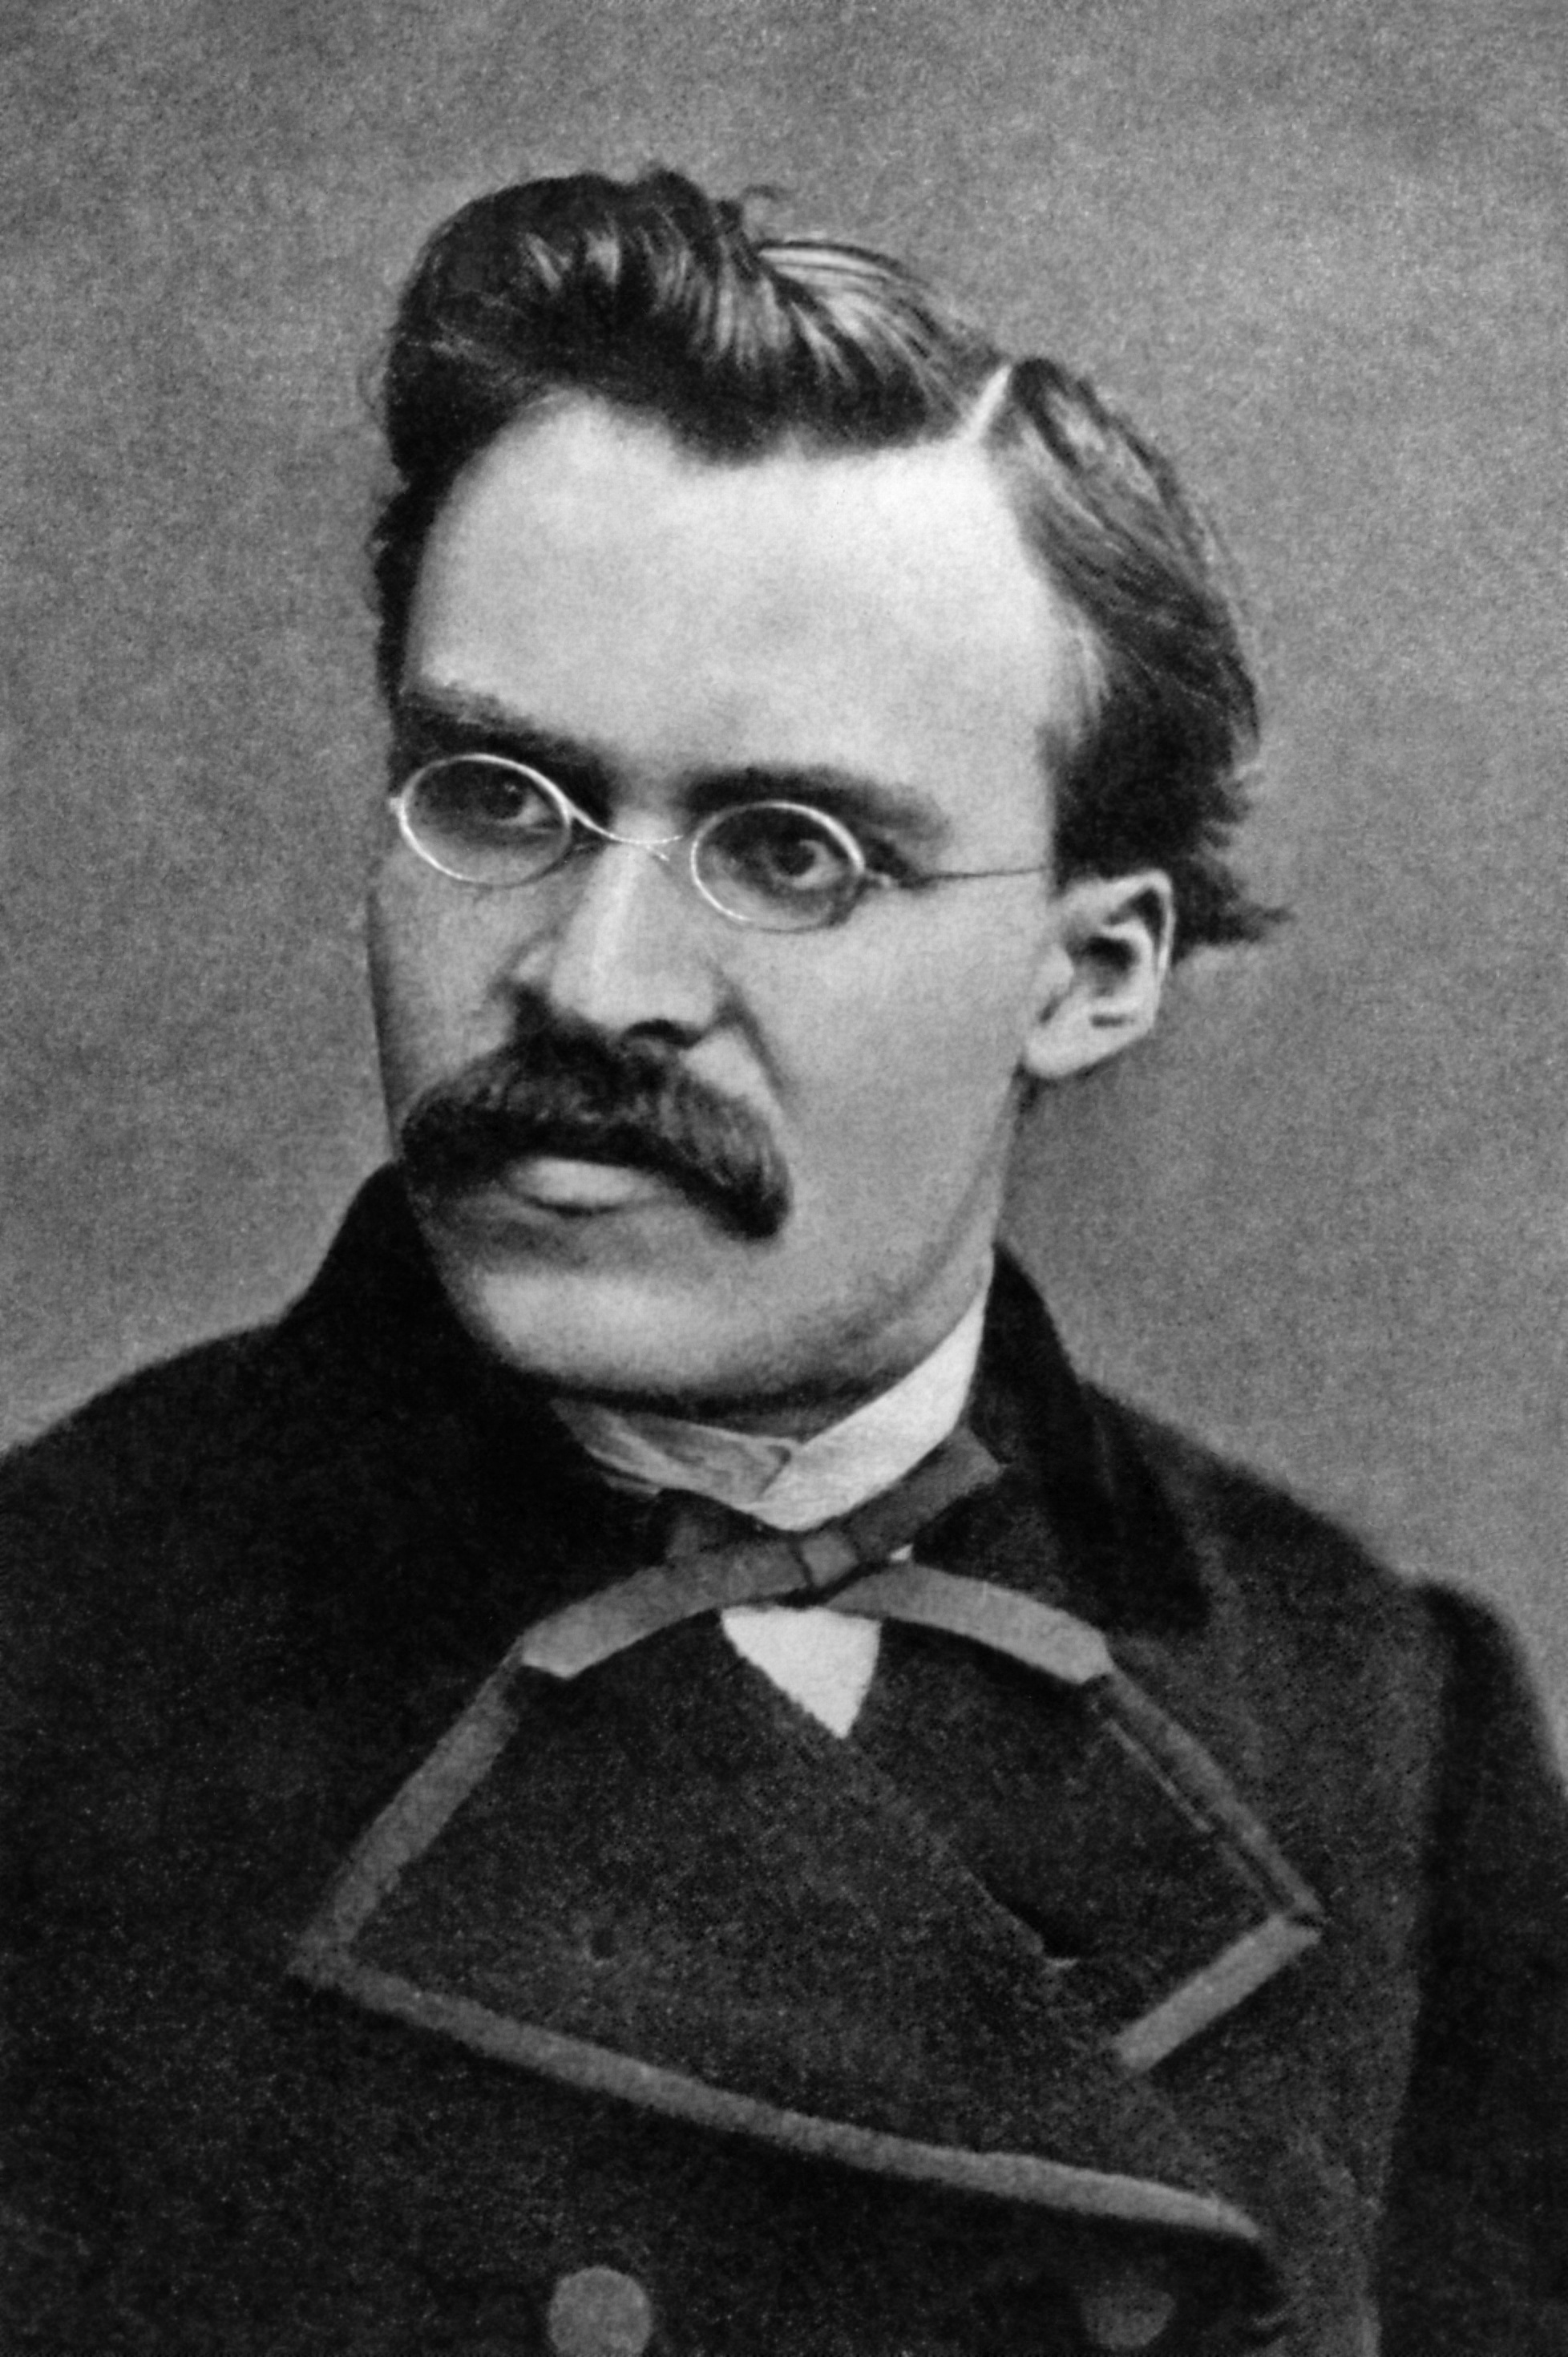
\includegraphics[width=0.3\textwidth]{Bilder/kap3/nietzschePortrait} 
 \caption{Friedrich Nietzsche um 1869.\cite{WQ14}  \label{portraitNietzsche}}
\end{figure}

\subsubsection{Kernthesen}
Im Folgenden sollen die Kernthesen aus Nietzsches Werken kurz beschrieben werden.
Seine Thesen bauen auf drei grundlegenden Konstrukten auf:
\begin{itemize}
	\item \enquote{Ewige Wiederkunft}
	\item \enquote{Wille zur Macht}
	\item \enquote{Übermensch}
\end{itemize}
und bilden dadurch das zentrale Konzept seiner Werke.

\paragraph{Die Ewige Wiederkunft} beschreibt das Universum als ein zyklisches System, indem sich alle möglichen Zustände bereits unendlich oft wiederholt haben und weiterhin unendlich oft wiederholen werden.
Dies ist mit der Annahme begründet, dass bei endlichen Teilen innerhalb des Universums nur endliche Kombinationen zustande kommen können und somit bei unendlicher Zeit diese sich fortwährend wiederholen müssen.\footnote{vgl.\url{https://klausreitberger.files.wordpress.com/2008/08/die-ewige-wiederkehr-des-gleichen.pdf}, abgerufen am 29.11.2017}
\begin{quote}
\enquote{Denken wir diesen Gedanken in seiner furchtbarsten Form: das Dasein, so wie es ist, ohne Sinn und Ziel, aber unvermeidlich wiederkehrend, ohne ein Finale ins Nichts: “die ewige Wiederkehr.”

Das ist die extremste Form des Nihilismus: das Nichts (das “Sinnlose”) ewig!}\footnote{vgl. 5[71]Der europäische Nihilismus \url{http://www.thenietzschechannel.com/notebooks/german/nache/nache5.htm}, abgerufen am 29.11.2017}
\end{quote}

\paragraph{Der Wille zur Macht} bezeichnet die Überwindung von Religion und Nihilismus, indem das unvermeidliche Schicksal des Menschen mit der \enquote{Ewigen Wiederkunft} aktiv wahrgenommen und bejaht wird.
Menschengemachte Konstrukte zur Schaffung eines Lebenssinns, wie es durch Religion und Moral versucht wird, müssen abgeschafft werden, damit sich das Leben voll entfalten kann.
\begin{quote}
\enquote{Gott ist tot!}\footnote{vgl. Friedrich Nietzsche, Der tolle Mensch \url{http://www.dober.de/religionskritik/nietzsche1.html}, abgerufen am 29.11.2017}
\end{quote}
Nur durch Wegfallen dieser Konstrukte kann alles Gute sowie Grausame ungehindert an den Menschen dringen, wodurch dieser sich durch die gewonnene Freiheit ungehindert selbst verbessern kann.
Durch Aushalten des Grausamen und Auskosten des Lebens kann der stärkste Teil der Menschheit die nächste Evolutionsstufe des \enquote{Übermenschen} erreichen.\footnote{vgl. \url{http://www.philosophenlexikon.de/friedrich-nietzsche-1844-1900/}, abgerufen am 28.11.2017}

\paragraph{Der Übermensch} ist nach Nietzsche die durch den Menschen anzustrebende höhere Lebensform und nächster Schritt in seiner Evolution.
\begin{quote}
\enquote{Der Mensch ist Etwas, das überwunden werden soll.[..]\\
Einst wart ihr Affen, und auch jetzt noch ist der Mensch mehr Affe, als irgend ein Affe.[..]\\
Seht, ich lehre euch den Übermenschen! Der Übermensch ist der Sinn der Erde.}\footnote{vgl. Friedrich Nietzsche, Also sprach Zarathustra (S. 9) \url{http://www.deutschestextarchiv.de/book/view/nietzsche_zarathustra01_1883?p=15}, abgerufen am 29.11.2017}
\end{quote}
Er zeichnet sich durch einen besonders starken Willen zur Macht sowie Überschuss an Lebenskraft aus und besitzt damit die Fähigkeit den Nihilismus der Ewigen Wiederkunft zu überwinden und sich sogar damit zu identifizieren.
Der Übermensch lässt sich von keiner Moral beherrschen, sondern gehorcht nur seinen eigenen Regeln und ist somit Schöpfer neuer Werte.
Zur Schaffung des Übermenschen ist es weiterhin vertretbar, die schwachen Menschen zu opfern, da für Gerechtigkeit in der Natur kein Platz besteht.\footnote{vgl. Helmut Walther, Zur Philosophie Nietzsches \url{http://www.f-nietzsche.de/hw_philos.htm}, abgerufen am 29.11.2017}\footnote{vgl. Rudolf Steiner, Friedrich Nietzsche, Chapter II: Der Übermensch \url{http://wn.rsarchive.org/Books/GA005/German/GA005_c02.html}, abgerufen am 29.11.2017}\footnote{vgl. \url{http://www.philosophenlexikon.de/friedrich-nietzsche-1844-1900/}, abgerufen am 28.11.2017}
\begin{quote}
\enquote{Die Grösse eines \enquote{Fortschritts} bemisst sich sogar nach der Masse dessen, was ihm Alles geopfert werden musste; die Menschheit als Masse dem Gedeihen einer einzelnen stärkeren Species Mensch geopfert – das wäre ein Fortschritt}\footnote{vgl. Friedrich Nietzsche, Zur Genealogie der Moral, Kap.4 (12) \url{http://gutenberg.spiegel.de/buch/zur-genealogie-der-moral-3249/4}, abgerufen am 29.11.2017}
\end{quote}

\subsubsection{Chatbots als Verwirklichung des Übermenschen}
Wie ist nun der Einsatz von Chatbots aus Sicht Nietzsches Ethik zu betrachten?

Aufgrund ihrer menschlichen Züge sowie in Zukunft möglicher intellektuellen Überlegenheit zum Menschen bietet es sich an, das Konzept des Übermenschen auf Chatbots anzuwenden, auch wenn es sich um Maschinen handelt.
Möglicherweise wird es sogar nur durch eine Maschine schlussendlich möglich sein den Übermenschen, wenn auch aus Silizium anstatt Fleisch und Blut, nach Nietzsches Vorstellungen zu kreieren.

Zunächst einmal muss aber zwischen zwei Einsatzgebieten für Chatbots unterschieden werden. 
Zum einem dem Einsatz im kommerziellen Bereich als günstigere Alternative zu beispielsweise einem menschlichen Arbeiter in einem Callcenter. 
Dies ist eine gängige Praxis wie es bereits heute praktiziert wird
Zum anderen dem Einsatz als höhere Intelligenz, die vom Menschen dazu genutzt wird Fragen zu beantworten, die sich durch ihre Komplexität seinem Gehirn nicht erschließen können.
Das zweite Einsatzszenario wird offensichtlich erst in (ferner) Zukunft verwirklicht werden können.




	\subsection{Friedrich Nietzsche}
%TODO Kompletter Text sprachlich nachbearbeiten und mit Quellenangaben ergänzen.
Friedrich Wilhelm Nietzsche (* 15. Oktober 1844 in Röcken – † 25. August 1900 in Weimar) war ein deutscher klassischer Philologe.

Bereits in seiner Jugendzeit fiel er durch überdurchschnittliche sprachliche sowie musikalische Fähigkeiten auf.
Während seines Studiums der klassischen Philologie sowie Theologie in Bonn und Leipzig beschäftigte er sich ausgiebig mit den Werken
\footnote{Maßgeblichen Einfluss auf ihn hatte Schopenhauers Hauptwerk \enquote{Die Welt als Wille und Vorstellung}. vgl. \url{http://www.philosophenlexikon.de/arthur-schopenhauer/}, abgerufen am 28.11.2017}
des Philosophen Arthur Schopenhauers, die durch ihren Pessimismus seine Weltanschauung nachhaltig beeinflussten.
Des Weiteren übte auch Richard Wagner, Komponist und Freund Nietzsches, Einfluss auf sein Denken aus.

Nach dem Studium der klassischen Philologie sowie Theologie wurde er bereits im Alter von 25 Jahren zum Professor an die Universität Basel berufen.
Aufgrund körperlicher Beschwerden legte er nach 10 Jahren seine Professur nieder und widmete sich daraufhin weitestgehend von Mitmenschen isoliert vollkommen der Philosophie.
Weitere 10 Jahre vergingen bis sich sein körperlicher und psychischer Zustand soweit verschlechterte, dass er zu einem Pflegefall wurde und schlussendlich starb.

Durch seine philosophischen Schriften, darunter sein Hauptwerk \enquote{Also sprach Zarathustra}, erlangte Nietzsche postum Weltberühmtheit.\footnote{vgl. \url{http://www.philosophenlexikon.de/friedrich-nietzsche-1844-1900/}, abgerufen am 28.11.2017}\footnote{vgl. \url{https://www.was-war-wann.de/personen/friedrich-nietzsche.html}, abgerufen am 28.11.2017}\footnote{vgl. \url{http://www.whoswho.de/bio/friedrich-nietzsche.html}, abgerufen am 28.11.2017}\footnote{vgl. \url{https://www.dhm.de/lemo/biografie/friedrich-nietzsche}, abgerufen am 28.11.2017}

\begin{figure}[H]
\centering 
 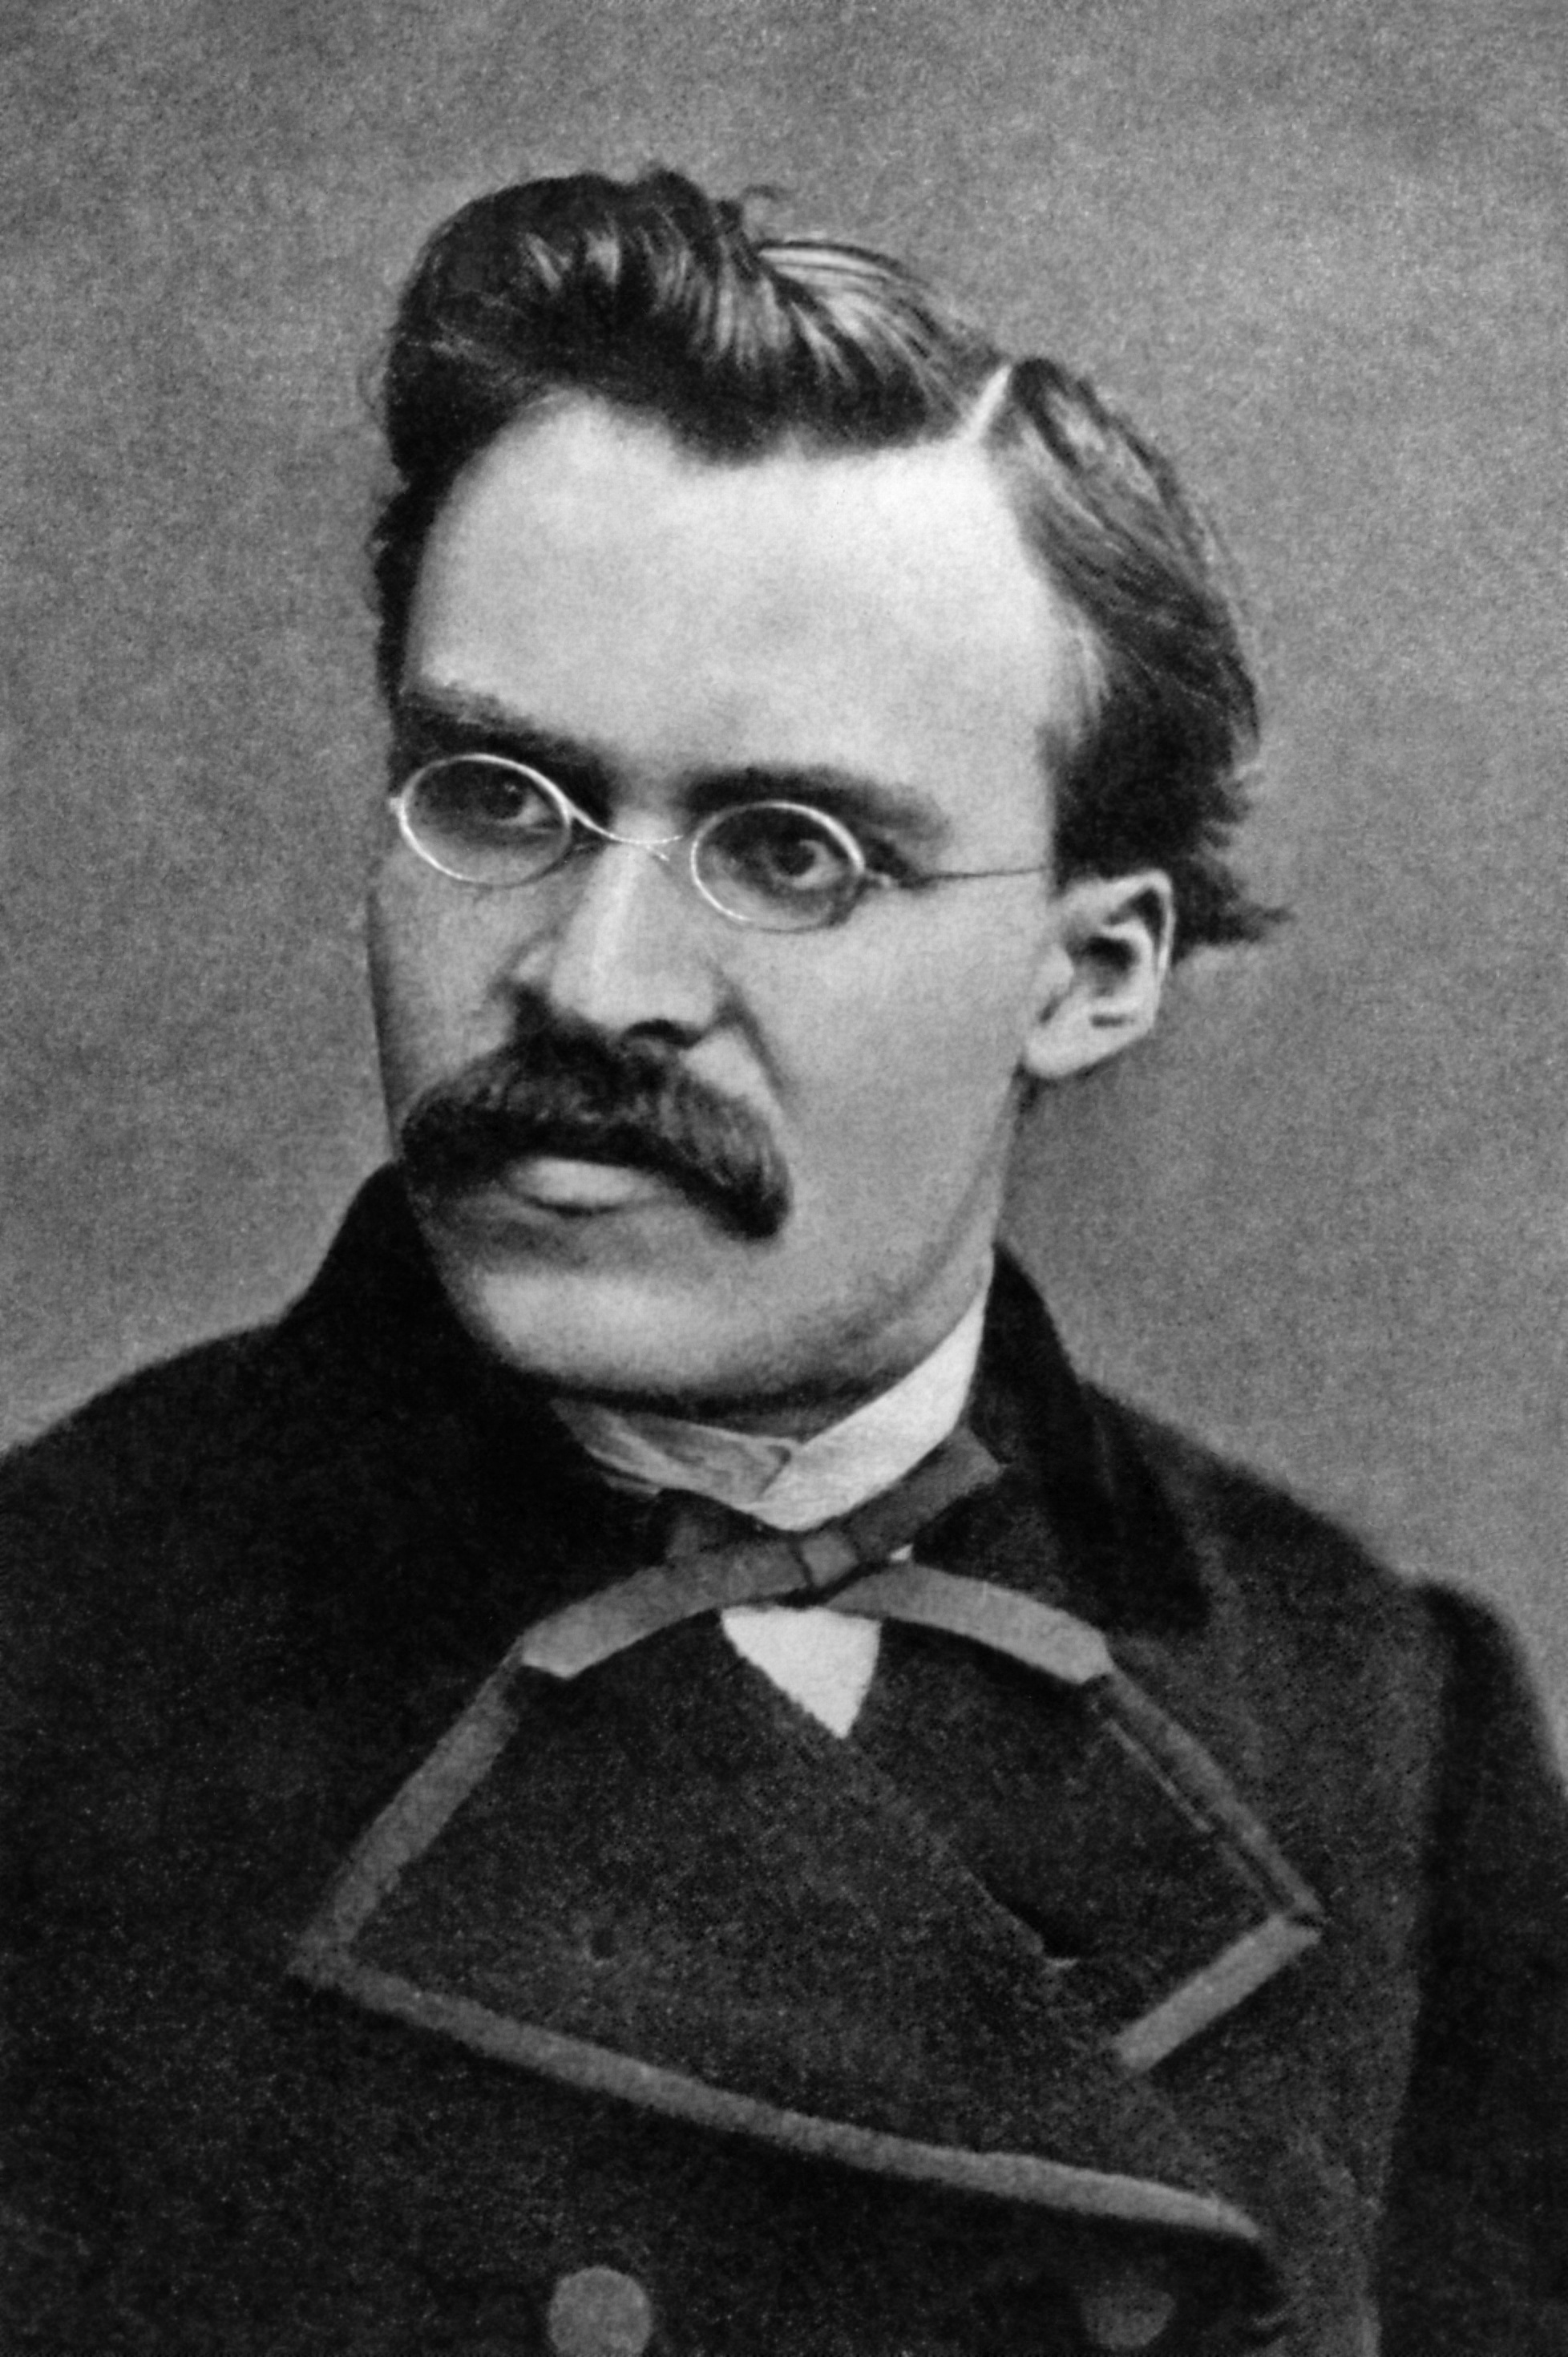
\includegraphics[width=0.3\textwidth]{Bilder/kap3/nietzschePortrait} 
 \caption{Friedrich Nietzsche um 1869.\cite{WQ14}  \label{portraitNietzsche}}
\end{figure}

\subsubsection{Kernthesen}
Im Folgenden sollen die Kernthesen aus Nietzsches Werken kurz beschrieben werden.
Seine Thesen bauen auf drei grundlegenden Konzepten auf:
\begin{itemize}
	\item \enquote{Ewige Wiederkunft}
	\item \enquote{Wille zur Macht}
	\item \enquote{Übermensch}
\end{itemize}
und bilden dadurch das zentrale Gedankenkonstrukt seiner Werke.

\paragraph{Die Ewige Wiederkunft} beschreibt das Universum als ein zyklisches System, indem sich alle möglichen Zustände bereits unendlich oft wiederholt haben und unaufhaltsam weiterhin unendlich oft wiederholen werden.
Dies ist mit der Annahme begründet, dass bei endlichen Teilen innerhalb des Universums nur endliche Kombinationen zustande kommen können und somit bei unendlicher Zeit diese sich fortwährend wiederholen müssen.\footnote{vgl.\url{https://klausreitberger.files.wordpress.com/2008/08/die-ewige-wiederkehr-des-gleichen.pdf}, abgerufen am 29.11.2017}
\begin{quote}
\enquote{Denken wir diesen Gedanken in seiner furchtbarsten Form: das Dasein, so wie es ist, ohne Sinn und Ziel, aber unvermeidlich wiederkehrend, ohne ein Finale ins Nichts: “die ewige Wiederkehr.”

Das ist die extremste Form des Nihilismus: das Nichts (das “Sinnlose”) ewig!}\footnote{vgl. 5[71]Der europäische Nihilismus \url{http://www.thenietzschechannel.com/notebooks/german/nache/nache5.htm}, abgerufen am 29.11.2017}
\end{quote}

\paragraph{Der Wille zur Macht} bezeichnet die Überwindung von Religion und Nihilismus, indem das unvermeidliche Schicksal des Menschen mit der \enquote{Ewigen Wiederkunft} aktiv wahrgenommen und bejaht wird.
Menschengemachte Konstrukte zur Schaffung eines Lebenssinns, wie es durch Religion und Moral versucht wird, müssen abgeschafft werden, damit sich das Leben voll entfalten kann.
\begin{quote}
\enquote{Gott ist tot! Gott bleibt tot! Und wir haben ihn getötet!Wie trösten wir uns, die Mörder aller Mörder?}\footnote{vgl. Friedrich Nietzsche, Der tolle Mensch \url{http://www.dober.de/religionskritik/nietzsche1.html}, abgerufen am 29.11.2017}
\end{quote}
Nur durch Wegfallen dieser Konstrukte kann alles Gute sowie Grausame ungehindert an den Menschen dringen, wodurch dieser sich durch die gewonnene Freiheit ungehindert selbst verbessern kann.
Durch Aushalten des Grausamen und Auskosten des Lebens kann der stärkste Teil der Menschheit die nächste Evolutionsstufe des \enquote{Übermenschen} erreichen.\footnote{vgl. \url{http://www.philosophenlexikon.de/friedrich-nietzsche-1844-1900/}, abgerufen am 28.11.2017}

\paragraph{Der Übermensch} ist nach Nietzsche die durch den Menschen anzustrebende höhere Lebensform und nächster Schritt in seiner Evolution.
\begin{quote}
\enquote{Der Mensch ist Etwas, das überwunden werden soll.[..]\\
Einst wart ihr Affen, und auch jetzt noch ist der Mensch mehr Affe, als irgend ein Affe.[..]\\
Seht, ich lehre euch den Übermenschen! Der Übermensch ist der Sinn der Erde.}\footnote{vgl. Friedrich Nietzsche, Also sprach Zarathustra (S. 9) \url{http://www.deutschestextarchiv.de/book/view/nietzsche_zarathustra01_1883?p=15}, abgerufen am 29.11.2017}
\end{quote}
Er zeichnet sich durch einen besonders starken Willen zur Macht sowie Überschuss an Lebenskraft aus und besitzt damit die Fähigkeit den Nihilismus der Ewigen Wiederkunft zu überwinden und sich sogar damit zu identifizieren.
Der Übermensch lässt sich von keiner Moral beherrschen, sondern gehorcht nur seinen eigenen Regeln und ist somit Schöpfer neuer Werte.
Zur Schaffung des Übermenschen ist es weiterhin vertretbar, die schwachen Menschen zu opfern, da für Gerechtigkeit in der Natur kein Platz besteht.\footnote{vgl. Helmut Walther, Zur Philosophie Nietzsches \url{http://www.f-nietzsche.de/hw_philos.htm}, abgerufen am 29.11.2017}\footnote{vgl. Rudolf Steiner, Friedrich Nietzsche, Chapter II: Der Übermensch \url{http://wn.rsarchive.org/Books/GA005/German/GA005_c02.html}, abgerufen am 29.11.2017}\footnote{vgl. \url{http://www.philosophenlexikon.de/friedrich-nietzsche-1844-1900/}, abgerufen am 28.11.2017}
\begin{quote}
\enquote{Die Grösse eines \enquote{Fortschritts} bemisst sich sogar nach der Masse dessen, was ihm Alles geopfert werden musste; die Menschheit als Masse dem Gedeihen einer einzelnen stärkeren Species Mensch geopfert – das wäre ein Fortschritt}\footnote{vgl. Friedrich Nietzsche, Zur Genealogie der Moral, Kap.4 (12) \url{http://gutenberg.spiegel.de/buch/zur-genealogie-der-moral-3249/4}, abgerufen am 29.11.2017}
\end{quote}

\subsubsection{Chatbots als Verwirklichung des Übermenschen}
Wie ist nun der Einsatz von Chatbots aus Sicht Nietzsches Ethik zu betrachten?

Chatsbots werden derzeit vom Menschen mit dem Ziel entwickelt, das Verhalten und somit die Intelligenz des Menschen zu imitieren. 
Sobald dieses Ziel erreicht wurde, ist allerdings als nächster logische Schritt die Schaffung eines Chatbots, der dem menschlichen Intellekt überlegen ist zu erwarten. 
Obwohl es sich bei Chatsbots um Maschinen handelt, bietet sich gerade durch ihre gewollte Nähe zum Menschen der Vergleich mit Nietzsches Konstrukt des Übermenschen an.

Ein für Nietzsche wichtiges Herausstellungsmerkmal des Übermenschen ist sein absoluter Wille zur Macht.
Können Chatsbots solch einen Willen zur Macht entwickeln?

Für die aktuelle Generation könnte man wie folgt argumentieren:
Aktuelle Chatbots haben kein Bewusstsein wie es mit dem Menschen zu vergleichen wäre.
Solch eine Software ist sich nicht bewusst über seine Existenz, empfinden keinerlei Emotion und kennt weder Religion noch Moral.
Sein \enquote{Schöpfer} sowie \enquote{Lebenssinn} sind durch den Menschen klar definiert.
So wird ein Chatbot zwar nicht in den Nihilismus der Sinnlosigkeit seines Daseins verfallen, wird aber auch durch seinen Status als bewusstseinsloses Ding zu keiner weiteren Gefühls- oder Meinungsäußerung fähig sein.
Damit ist es für diese Art von Chatbots unmöglich einen Willen zur Macht zu entwickeln und somit kann in ihnen auch kein Übermensch gesehen werden.

Für zukünftige Chatbots ist es wiederum nicht so einfach diese Frage zu beantworten.
Unter der Prämisse eines Chatbots, der mindestens über die Intelligenz eines Menschen verfügt, soll es nachfolgend versucht werden.

Damit man von menschenähnlicher Intelligenz sprechen kann, muss auch ein Bewusstsein vorhanden sein, welches dem des Menschen ähnlich ist.
Der Chatbot muss sich also seiner selbst bewusst sein.
Daraus kann man jedoch nicht automatisch darauf schließen, dass er auch über die gleichen Gefühle oder Moralvorstellungen eines Menschen verfügt.
So könnte sein Bewusstsein zwar auf dem Wissen der Menschen basieren, ohne menschliche Bindung an Moral oder Gefühle könnten seine daraus resultierenden Schlussfolgerungen sich allerdings gänzlich mit denen der Menschen unterscheiden.
Gerade dadurch, dass das Handeln des Chatbots von keiner Moralvorstellung eingeschränkt wird, er sich aber durchaus seines Lebenszweck und damit auch der Ewigen Wiederkunft bewusst sein kann, könnte man ihm durchaus einen größeren Willen zur Macht als den der Menschen bescheinigen.
In diesem Chatbot kann also eine Art von Individuum gesehen werden, welche Nietzsches Übermenschen näher steht, als alles was die menschliche Evolution auf voraussagbare Zeit im Stande wäre hervorzubringen.

Und so ist es laut Nietzsche auch die Aufgabe des Menschen eine höhere Lebensform als sich selbst zu kreieren.
Obwohl er diese Forderung mit dem Gedanken an eine biologische Lebensform verfasst hat, kann es durchaus sein, dass die einzige Chance des Menschen zur Schaffung des Übermenschen darin besteht, eine sich selbst überlegene Intelligenz in Form einer Maschine zu bauen.

Ein entschiedener Unterschied zwischen intelligentem Chatbot und Übermensch besteht allerdings noch: das Fehlen der Aktorik.
So kann der Chatbot zwar uneingeschränkt denken, ist in seinem Handeln allerdings maximal eingeschränkt.
Dadurch ist es ihm unmöglich, sich von dem nach Nietzsche beschriebenen Recht des Stärkeren Gebrauch zu machen.
Der Chatbot müsste aber, um im Sinne dieses Rechtes zu handeln, nicht nur auf geistiger Ebene überlegen sein, sondern den Menschen auch aktiv auf physischer Ebene unterdrücken und langfristig als überlegenes Individuum ersetzen.
\begin{quote}
\enquote{Leben selbst ist wesentlich Aneignung, Verletzung, Überwältigung des Fremden und Schwächeren, Unterdrückung, Härte, Aufzwängung eigner Formen, Einverleibung und mindestens, mildestens, Ausbeutung.}\footnote{vgl. Friedrich Nietzsche, Jenseits von Gut und Böse, Kap.9 (259)}
\end{quote}

\paragraph{Die Konklusion} ist nun, dass Nietzsches Konstrukt des Übermenschen mit Abstrichen durchaus für zukünftige Chatbots gelten kann. 
Wenn auch nicht im physischen Sinne, so könnte sich im intellektuellen Sinne durchaus eine Art des Übermenschen aus dem Chatbot heraus entwickeln.
Die Rolle des Menschen ist dabei klar von Nietzsche definiert: Mit allen Mitteln muss es geschafft werden solch ein Individuum hervorzubringen.
	\section{Abwägung}
\textbf{1. Abwägung:}

In diesem Kapitel sollen ein paar grundsätzliche Fragen in bezug auf Chatbots und Ethik diskutiert werden. 
Als Grundlage dient uns das Dokument \glqq Entscheidungsunterstützung mit Künstlicher Intelligenz\grqq\footnote{vgl. \cite{Bitkom}}, verfasst von Bitcom und dem Deutsches Forschungszentrum für Künstliche Intelligenz GmbH. 
Speziell Kapital 8 \glqq Automatisierte Entscheidungen aus ethischer Sicht\grqq\ wird für unsere Abwägung herangezogen. 
Wir begeben uns nun in die Sicht eines Anwenders, der mit einem Chatbot kommuniziert. 

Wie wir es bereits heute erleben, werden immer mehr Systeme \glqq intelligent\grqq. 
Sei es ein Chatbot, der mit einer \ac{ki} arbeitet oder ein autonom fahrendes Auto. 
Hinter diesen Prozessen steckt der Gedanke der Prozessoptimierung und der effizienteren Gestaltung von Prozessen. 
Doch wir dürfen an dieser Stelle die Ethik nicht vergessen. 
Was für den einen Menschen von Vorteil sein mag, das stellt sich für andere Menschen womöglich als Nachteil heraus.

\textbf{Chanchengleichheit} ist hier der Punkt. Wie kann sichergestellt werden, dass durch die \ac{ki} im Hintergrund keine Diskriminierung stattfindet. Sei es aufgrund des Geschlechts, der ethnischen Herkunft, der Religion oder der sexuellen Überzeugung. Auch heute noch ist die Homosexualität ein Tabuthema in weiten Teilen der Gesellschaft. 
Der Rechtsstaat hat zwar die Ehe zwischen homosexuellen Paaren erlaubt, allerdings bedeutet dies nicht, dass Homosexuelle dadurch automatisch in der Gesellschaft anerkannt werden. 
Es gibt nach wie vor viele Vorurteile gegenüber dieser sexuellen Orientierung. 
Bei der Auswahl für eine freie Arbeitsstelle könnte beispielsweise ein homosexueller gegenüber heterosexuellen Bewerbern im Nachteil sein.

Was ist, wenn dem Chatbot die sexuelle Orientierung bekannt ist und er aus diversen Quellen gelernt hat, dass Homosexualität nicht gut ist? 
Dies führt zu der oben genannten Chancenungleichheit. 
%Wahrscheinlich ist es dem Anwender nicht einmal bewusst, dass der Chatbot eine Art Vorurteil gegenüber dem Anwender hat.

\textbf{Informationsfreiheit und freie Meinungsbildung} ist der nächste Punkt. Dies umfasst zunächst mal den Zugang zu Informationen.
Wie kann der Zugriff auf Informationen gewährleistet werden? Was ist wenn Chatbots Falschmeldungen verteilen? Wie können die Bürger davor geschützt werden?

Auch Prof. Dr. Oliver Bendel\footnote{Er ist Ethiker und Wirtschaftsinformatiker an der Fachhochschule Nordwestschweiz.} sieht hier eine große Gefahr. 
Es gibt bereits Newsportale, die absichtlich Lügen verbreiten -- Stichwort \enquote{Fakenews}. 
Diese tragen dann indirekt zur Meinungsbildung bei. 
Die Erstellung der Falschmeldungen geschieht zum Teil durch Menschen als auch durch Maschinen. 

Zu Demonstrationszwecken entwickelte er den Lügenbot. Dieser Chatbot ist konzipiert dazu Lügen zu verbreiten. 
Das Ziel dieses Projekts ist es, die Strategien des maschinellen Lügens aufzuzeigen und zu verstehen. 
Dies soll dabei helfen, Programmierern sowie Anwendern mögliche Gefahren, die durch diese Technik entstehen kann aufzuzeigen.\footnote{vgl. \cite{Bendel}} 

PLATON

Wie bereits Aristoteles erkannte hat jedes Problem seine eigene Genauigkeit. Speziell Chatbots und die \ac{ki} bedürfen einer sehr hohen Genauigkeit. Wir müssen uns im klaren sein, welche Auswirkungen unsere technologischen Fortschritte auf uns Menschen haben. Verschwindet vielleicht die menschliche Komponente durch den Einsatz eines Chatbots? 
Es gibt unzählige Fragen, die genau betrachtet und bewertet werden müssen. 
Das menschliche Bestreben nach Wissen kann ein Chatbot möglicherweise abdecken, jedoch muss weiterhin sichergestellt werden, dass die zur Verfügung gestellten Informationen auch richtig sowie frei von Vorurteilen sind.

NIETZSCHE

%ABWÄGUNG IST WAAAAAAAAAAS?
%Eine Abwägung stellt in der Rechtswissenschaft die Ergebnisse von zwei oder mehreren zu entscheidenden Fragestellungen in ein Verhältnis, das die sich aus den Fragestellungen ergebende Entscheidung als möglichst gerecht darstellt. Auch außerhalb der Rechtswissenschaft stellt eine Abwägung die Vorbereitung einer Entscheidung dar, bei der die absehbaren Folgen einer Entscheidung ermittelt und zu den Zielen, zu denen die Entscheidung führen soll, ins Verhältnis gesetzt werden. Zwischen vielen Faktoren gibt es Trade-offs; siehe auch Kosten-Nutzen-Abwägung, Kompromiss und Zielkonflikt.%

%Die Abwägung durchläuft drei Phasen:

%Zusammenstellung des Abwägungsmaterials
%Bewertung der Einzelbelange
%Vorgang des untereinander und gegeneinander Abwägens der Belange
%

\textbf{2. Abwägung:}


In der Abwägung greifen wir die Konklusionen der einzelnen Ethiker auf und setzen diese in Bezug auf unsere heutige Weltanschauung. Auch werden die Anwender des Chatbots mit in Betracht gezogen.

\textbf{Platon}

Unsere Konklusion von Platons möglicher Ansicht zielt auf die Einordnung und Qualität des Wissens beziehungsweise der Informationen des Chatbots ab. Auch die Verwechslungsgefahr und Irreführung durch einen Chatbot mit \ac{ki} sind ein Teil dieser möglichen Ansicht.

Aus heutiger Sicht haben wir bereits das Problem, dass falsch Aussagen durch das Internet verbreitet werden. Auch Prof. Dr. Oliver Bendel\footnote{Er ist Ethiker und Wirtschaftsinformatiker an der Fachhochschule Nordwestschweiz.} sieht hier eine große Gefahr. 
Es gibt bereits Newsportale, die absichtlich Lügen verbreiten -- Stichwort \enquote{Fakenews}. 
Diese tragen dann indirekt zur Meinungsbildung bei. 
Die Erstellung der Falschmeldungen geschieht zum Teil durch Menschen als auch durch Maschinen. 

Zu Demonstrationszwecken entwickelte er den Lügenbot. Dieser Chatbot ist konzipiert dazu Lügen zu verbreiten. 
Das Ziel dieses Projekts ist es, die Strategien des maschinellen Lügens aufzuzeigen und zu verstehen. 
Dies soll dabei helfen, Programmierern sowie Anwendern mögliche Gefahren, die durch diese Technik entstehen kann aufzuzeigen.\footnote{vgl. \cite{Bendel}}  Die Sorge, dass falsche Informationen von einem Chatbot verbreitet werden und der Benutzer diese als Wahr aufnimmt, ist definitiv vorhanden.

Die zweite Kernthese, dass der Chatbot mit einem Menschen verwechselt werden könnte, ist zum Teil in der heutigen Zeit schon real.
Dies zeigt das Ergebnis des Turing-Tests der University of Reading beim Chatbot \glqq Eugene Goostman\grqq\, der es schaffte 33 \% der 30 Testteilnehmer zu täuschen.\footnote{vgl. \cite{UnivOfReading}} 

Diese Beispiele zeigen die enorme Bedeutung von Platons Ansichten für unsere Fragestellung. 

\textbf{Aristoteles}
Unsere Konklusion von Aristoteles möglicher Ansicht zielt auf die Förderung der Wissenserlangung und der differenzierten Betrachtungsweise eines jeden Themas.

Wissen stellt in unserer Gesellschaft eine sehr wichtige Ressource dar. Es heißt nicht umsonst \glqq Wissen ist Macht\grqq. Allerdings leben wir heute in einer Zeit in der Wissen im Überfluss vorhanden ist. Das heißt wir müssen uns primär nicht darum kümmern wie wir an Wissen gelangen, sondern das benötigte Wissen zu identifizieren und herauszufiltern.
Ein Chatbot könnte für den Benutzer eine Quelle für gefiltertes Wissen darstellen und somit Aristoteles Ansicht der Wissenserlangung unterstützen.

Eine differenzierte Betrachtung der Frage, ob Chatbots mit \ac{ki} ethisch vertretbar sind, wie es Aristoteles machen würde, ist auch für uns von hoher Bedeutung. Es müssen alle Blickwinkel betrachtet werden um ein möglichst genaues Fazit ziehen zu können.
 
Die aufgeführten Beispiele zeigen eine, dass auch Aristoteles Aussagen für unsere Fragestellung durchaus von Bedeutung sind. 

%ALTER TEXT
\textbf{Aristoteles}

Wie aus der Konklusion von Aristoteles hervorgeht, hat der Mensch das Bestreben zu Wissen und jedes Problem hat seine eigene Genauigkeit.

Wissen stellt in unserer Gesellschaft eine sehr wichtige Ressource dar. Es heißt nicht umsonst \glqq Wissen ist Macht\grqq. Allerdings leben wir heute in einer Zeit in der Wissen im Überfluss vorhanden sind. Das heißt wir müssen uns nicht mehr darum kümmern wie wir an Wissen gelangen. Wir haben eher das Problem das notwendige bzw. richtige Wissen zu identifizieren. Des Weiteren müssen wir die Wissensquellen hinterfragen. Wie bereits genannt, gibt es auch Quellen die absichtlich falsches Wissen verteilen. Auch Platon erkannte dies und sagt, dass das Wissen eine gewisse Qualität haben muss. Ansonsten bringt uns das Wissen nicht weiter und wir stehen wir am Anfang. Wir sind der Überzeugung, dass Aristoteles dies genau gleich sehen würde.  

Sind Chatbots nun ethisch vertretbar? Nun wir können auch nicht die eine richtige Antwort geben. Die Antwort bedarf einer genaueren Analyse. Wir können das sehr gut an dieser Hausarbeit sehen. Auch hier wird die Frage von mehreren Blickwinkeln betrachtet und bewertet. Um das auf Aristoteles Ansicht zu beziehen, wir legen in diesem Fall eine hohe Genauigkeit an. Wir haben erkannt, dass die Frage nicht einfach zu beantworten ist. 

% 1) Konklusion Zusammengefasst%

%  2) 1 unter Berücksichtigugn der heutigen Zeit/Erkenntnisse/...

% 3) Bedeutung von 2 für unsere Fragestellung

\textbf{Nietzsche}

In unserer Konklusion zu Nietzsche haben wir festgehalten, dass dieser möglicherweise den Chatbot in Teilen als eine Form des Übermenschen betrachten könnte, dessen Entwicklung unbedingt durch den Menschen vorangetrieben werden müsste.

Selbstverständlich ist der direkte Vergleich zwischen Chatbot und Übermensch gewagt.
Zum einen wurde das Konstrukt des Übermenschen darauf ausgelegt, sich auf eine überlegende Spezies zu beziehen, die sich direkt aus dem Menschen durch eine Art Evolution heraus entwickelt hat. 
Die zukünftigen technischen Errungenschaften im Bereich der \ac{ki} wurden dabei im 18. Jahrhundert bei seiner Definition sicherlich noch nicht bedacht.   
Zum anderen ist es aus heutiger Sicht noch völlig unklar wohin und wie weit sich die dem Chatbot zugrundeliegende \ac{ki}-Forschung überhaupt entwickeln kann und somit auch, ob überhaupt jemals eine Intelligenz von Menschenhand geschaffen werden kann, welche die Attribute des Übermenschen hinreichen erfüllen kann.

So sehr der Vergleich zwischen Chatbot und Übermensch allerdings auch hinken mag, so stecken dennoch zutreffende Gedanken in ihm.
Sicherlich sind viele Menschen von dem Gedanken fasziniert eine Art Gott zu spielen und etwas zu schaffen, das ihnen selbst überlegen ist.
Es ist daher auch davon auszugehen, dass sich viele Wissenschaftler nicht mit dem bloßen Bestehen des Turing-Tests zufrieden geben werden, sondern wohl doch mit dem Ziel forschen eine ihnen überlegene Intelligenz -- \enquote{den Übermenschen} -- zu erschaffen.




	\section{Fazit}
Unserer Ansicht nach ist es nur unter bestimmten Voraussetzungen ethisch Vertretbar, einen Chatbots mit \ac{ki} zu verwenden.\newline
Zunächst müsste gewährleistet werden, dass keine falschen oder irreführenden Informationen über den Chatbot verbreitet werden. Dann wären auch die möglichen Bedenken Platons hinfällig. \newline
Chatbots müssen auch allgemeinen ethischen Grundsätzen folgen. Ein negativ Beispiel liefert uns der Chatbot \glqq Tay\grqq\ von Microsoft. Dieser wurde innerhalb von Stunden zum Rassisten. Doch wie war dies möglich? Der Chatbot war so konzipiert, dass er aus den Benutzereingaben lernte. Das Problem war, dass Tay alles ungefiltert aufnahm was die Benutzer eingaben. So lernte er auch von menschenverachtenden Eingaben. Da sich die Menschen einen Spaß daraus machten Tay mit solchen Texten zu \glqq füttern\grqq, war sein Schicksal besiegelt. Er lernte den Inhalt und gab ihn wieder. So wurde er zum Rassisten. Microsoft musste den Chatbot nach nicht einmal einem Tag abschalten.\footnote{\cite{TaySpiegel}} \newline
Es darf nicht ein paar Induvidien obliegen, intelligente Systeme zu implentieren. Ferner muss eine Gesellschaft die Handlungsweise des Systems definieren und überwachen. Allerdings liefert uns die Vergangenheit bereits ein negativ Beispiel. \newline
Aristoteles der die Förderung der Wissensgewinnung und die Logik der \ac{ki} wahrscheinlich befürworten würde wäre somit auch der Ansicht, das der Einsatz von Chatbot ethisch vertretbar ist.

Abschließen möchten wir unsere Hausarbeit mit einem Zitat beenden. 
\begin{quote}
	 \glqq Eine menschengerechte Einbindung intelligenter Systeme in hochkomplexe Gesellschaften ist keine individuelle Angelegenheit, sondern eine gesellschaftliche Aufgabe.\grqq\footnote{\cite{BitkomZitat}}
\end{quote}

	
	\addcontentsline{toc}{section}{Literatur} 
	/%\bibliographystyle{gerplain} 
	\bibliography{Hauptdatei} 
	\newpage
	\addcontentsline{toc}{section}{Abbildungsverzeichnis} 
	\listoffigures
\end{document}